% Options for packages loaded elsewhere
\PassOptionsToPackage{unicode}{hyperref}
\PassOptionsToPackage{hyphens}{url}
\PassOptionsToPackage{dvipsnames,svgnames,x11names}{xcolor}
%
\documentclass[
  letterpaper,
  DIV=11,
  numbers=noendperiod]{scrartcl}

\usepackage{amsmath,amssymb}
\usepackage{iftex}
\ifPDFTeX
  \usepackage[T1]{fontenc}
  \usepackage[utf8]{inputenc}
  \usepackage{textcomp} % provide euro and other symbols
\else % if luatex or xetex
  \usepackage{unicode-math}
  \defaultfontfeatures{Scale=MatchLowercase}
  \defaultfontfeatures[\rmfamily]{Ligatures=TeX,Scale=1}
\fi
\usepackage{lmodern}
\ifPDFTeX\else  
    % xetex/luatex font selection
\fi
% Use upquote if available, for straight quotes in verbatim environments
\IfFileExists{upquote.sty}{\usepackage{upquote}}{}
\IfFileExists{microtype.sty}{% use microtype if available
  \usepackage[]{microtype}
  \UseMicrotypeSet[protrusion]{basicmath} % disable protrusion for tt fonts
}{}
\makeatletter
\@ifundefined{KOMAClassName}{% if non-KOMA class
  \IfFileExists{parskip.sty}{%
    \usepackage{parskip}
  }{% else
    \setlength{\parindent}{0pt}
    \setlength{\parskip}{6pt plus 2pt minus 1pt}}
}{% if KOMA class
  \KOMAoptions{parskip=half}}
\makeatother
\usepackage{xcolor}
\setlength{\emergencystretch}{3em} % prevent overfull lines
\setcounter{secnumdepth}{-\maxdimen} % remove section numbering
% Make \paragraph and \subparagraph free-standing
\makeatletter
\ifx\paragraph\undefined\else
  \let\oldparagraph\paragraph
  \renewcommand{\paragraph}{
    \@ifstar
      \xxxParagraphStar
      \xxxParagraphNoStar
  }
  \newcommand{\xxxParagraphStar}[1]{\oldparagraph*{#1}\mbox{}}
  \newcommand{\xxxParagraphNoStar}[1]{\oldparagraph{#1}\mbox{}}
\fi
\ifx\subparagraph\undefined\else
  \let\oldsubparagraph\subparagraph
  \renewcommand{\subparagraph}{
    \@ifstar
      \xxxSubParagraphStar
      \xxxSubParagraphNoStar
  }
  \newcommand{\xxxSubParagraphStar}[1]{\oldsubparagraph*{#1}\mbox{}}
  \newcommand{\xxxSubParagraphNoStar}[1]{\oldsubparagraph{#1}\mbox{}}
\fi
\makeatother


\providecommand{\tightlist}{%
  \setlength{\itemsep}{0pt}\setlength{\parskip}{0pt}}\usepackage{longtable,booktabs,array}
\usepackage{calc} % for calculating minipage widths
% Correct order of tables after \paragraph or \subparagraph
\usepackage{etoolbox}
\makeatletter
\patchcmd\longtable{\par}{\if@noskipsec\mbox{}\fi\par}{}{}
\makeatother
% Allow footnotes in longtable head/foot
\IfFileExists{footnotehyper.sty}{\usepackage{footnotehyper}}{\usepackage{footnote}}
\makesavenoteenv{longtable}
\usepackage{graphicx}
\makeatletter
\def\maxwidth{\ifdim\Gin@nat@width>\linewidth\linewidth\else\Gin@nat@width\fi}
\def\maxheight{\ifdim\Gin@nat@height>\textheight\textheight\else\Gin@nat@height\fi}
\makeatother
% Scale images if necessary, so that they will not overflow the page
% margins by default, and it is still possible to overwrite the defaults
% using explicit options in \includegraphics[width, height, ...]{}
\setkeys{Gin}{width=\maxwidth,height=\maxheight,keepaspectratio}
% Set default figure placement to htbp
\makeatletter
\def\fps@figure{htbp}
\makeatother

\AtBeginDocument{\let\oldnotes\notes
\renewcommand{\notes}[1]{}}
\KOMAoption{captions}{tableheading}
\makeatletter
\@ifpackageloaded{tcolorbox}{}{\usepackage[skins,breakable]{tcolorbox}}
\@ifpackageloaded{fontawesome5}{}{\usepackage{fontawesome5}}
\definecolor{quarto-callout-color}{HTML}{909090}
\definecolor{quarto-callout-note-color}{HTML}{0758E5}
\definecolor{quarto-callout-important-color}{HTML}{CC1914}
\definecolor{quarto-callout-warning-color}{HTML}{EB9113}
\definecolor{quarto-callout-tip-color}{HTML}{00A047}
\definecolor{quarto-callout-caution-color}{HTML}{FC5300}
\definecolor{quarto-callout-color-frame}{HTML}{acacac}
\definecolor{quarto-callout-note-color-frame}{HTML}{4582ec}
\definecolor{quarto-callout-important-color-frame}{HTML}{d9534f}
\definecolor{quarto-callout-warning-color-frame}{HTML}{f0ad4e}
\definecolor{quarto-callout-tip-color-frame}{HTML}{02b875}
\definecolor{quarto-callout-caution-color-frame}{HTML}{fd7e14}
\makeatother
\makeatletter
\@ifpackageloaded{caption}{}{\usepackage{caption}}
\AtBeginDocument{%
\ifdefined\contentsname
  \renewcommand*\contentsname{Inhaltsverzeichnis}
\else
  \newcommand\contentsname{Inhaltsverzeichnis}
\fi
\ifdefined\listfigurename
  \renewcommand*\listfigurename{Abbildungsverzeichnis}
\else
  \newcommand\listfigurename{Abbildungsverzeichnis}
\fi
\ifdefined\listtablename
  \renewcommand*\listtablename{Tabellenverzeichnis}
\else
  \newcommand\listtablename{Tabellenverzeichnis}
\fi
\ifdefined\figurename
  \renewcommand*\figurename{Abbildung}
\else
  \newcommand\figurename{Abbildung}
\fi
\ifdefined\tablename
  \renewcommand*\tablename{Tabelle}
\else
  \newcommand\tablename{Tabelle}
\fi
}
\@ifpackageloaded{float}{}{\usepackage{float}}
\floatstyle{ruled}
\@ifundefined{c@chapter}{\newfloat{codelisting}{h}{lop}}{\newfloat{codelisting}{h}{lop}[chapter]}
\floatname{codelisting}{Listing}
\newcommand*\listoflistings{\listof{codelisting}{Listingverzeichnis}}
\makeatother
\makeatletter
\makeatother
\makeatletter
\@ifpackageloaded{caption}{}{\usepackage{caption}}
\@ifpackageloaded{subcaption}{}{\usepackage{subcaption}}
\makeatother

\ifLuaTeX
\usepackage[bidi=basic]{babel}
\else
\usepackage[bidi=default]{babel}
\fi
\babelprovide[main,import]{nswissgerman}
% get rid of language-specific shorthands (see #6817):
\let\LanguageShortHands\languageshorthands
\def\languageshorthands#1{}
\ifLuaTeX
  \usepackage{selnolig}  % disable illegal ligatures
\fi
\usepackage{bookmark}

\IfFileExists{xurl.sty}{\usepackage{xurl}}{} % add URL line breaks if available
\urlstyle{same} % disable monospaced font for URLs
\hypersetup{
  pdftitle={Der Einfluss von Computational Thinking auf das Lernen im Allgemeinen},
  pdfauthor={Jacques Mock Schindler},
  pdflang={de-CH},
  colorlinks=true,
  linkcolor={blue},
  filecolor={Maroon},
  citecolor={Blue},
  urlcolor={Blue},
  pdfcreator={LaTeX via pandoc}}


\title{Der Einfluss von Computational Thinking auf das Lernen im
Allgemeinen}
\usepackage{etoolbox}
\makeatletter
\providecommand{\subtitle}[1]{% add subtitle to \maketitle
  \apptocmd{\@title}{\par {\large #1 \par}}{}{}
}
\makeatother
\subtitle{Präsentation Abschlussarbeit GymInf}
\author{Jacques Mock Schindler}
\date{13. September 2024}

\begin{document}
\maketitle


\subsection{Ausgangspunkt}\label{ausgangspunkt}

Quintessenz aus 20 Jahren Unterrichtserfahrung:

\begin{tcolorbox}[enhanced jigsaw, opacityback=0, arc=.35mm, coltitle=black, opacitybacktitle=0.6, title={Schulische Rahmenbedinungen}, bottomrule=.15mm, colbacktitle=quarto-callout-note-color!10!white, toprule=.15mm, bottomtitle=1mm, breakable, toptitle=1mm, left=2mm, rightrule=.15mm, leftrule=.75mm, colframe=quarto-callout-note-color-frame, titlerule=0mm, colback=white]

Schule findet im Konjunktiv statt.

\end{tcolorbox}

\begin{tcolorbox}[enhanced jigsaw, opacityback=0, arc=.35mm, coltitle=black, opacitybacktitle=0.6, title={Korrektiv}, bottomrule=.15mm, colbacktitle=quarto-callout-tip-color!10!white, toprule=.15mm, bottomtitle=1mm, breakable, toptitle=1mm, left=2mm, rightrule=.15mm, leftrule=.75mm, colframe=quarto-callout-tip-color-frame, titlerule=0mm, colback=white]

\begin{itemize}
\tightlist
\item
  Möglichst konkrete Aufgabenstellungen
\item
  Reale Werkzeuge einsetzen
\end{itemize}

\end{tcolorbox}

Praktisch nichts ist absolut verbindlich. Persönliche Teilname am APU
Projekt von Stephan Schumann.

\subsection{Arbeitshypothese}\label{arbeitshypothese}

\begin{tcolorbox}[enhanced jigsaw, opacityback=0, arc=.35mm, coltitle=black, opacitybacktitle=0.6, title={Konkrete Aufgabenstellung}, bottomrule=.15mm, colbacktitle=quarto-callout-tip-color!10!white, toprule=.15mm, bottomtitle=1mm, breakable, toptitle=1mm, left=2mm, rightrule=.15mm, leftrule=.75mm, colframe=quarto-callout-tip-color-frame, titlerule=0mm, colback=white]

Programmieren

\end{tcolorbox}

\begin{tcolorbox}[enhanced jigsaw, opacityback=0, arc=.35mm, coltitle=black, opacitybacktitle=0.6, title={Reale Werkzeuge}, bottomrule=.15mm, colbacktitle=quarto-callout-tip-color!10!white, toprule=.15mm, bottomtitle=1mm, breakable, toptitle=1mm, left=2mm, rightrule=.15mm, leftrule=.75mm, colframe=quarto-callout-tip-color-frame, titlerule=0mm, colback=white]

VS Code und Kollegen

\end{tcolorbox}

Damit Probleme algorithmisch gelöst werden können, ist es erforderlich,
diese gedanklich zu durchdringen.\\
Wenn Schülerinnen und Schüler allgemeingültige Programme für die Lösung
einer bestimmten Kategorie von Problemen schreiben, findet eine solche
gedankliche Durchdringung statt. Dies ist eine Anwendung von
Computational Thinking im Sinne der aktuellen Auffassung dieses
Begriffes und führt zu einem tieferen Verständnis der so gelösten
Probleme und damit zu einem nachhaltigen Lernerfolg.

\subsection{Psychologische Grundlagen}\label{psychologische-grundlagen}

\begin{tcolorbox}[enhanced jigsaw, opacityback=0, arc=.35mm, coltitle=black, opacitybacktitle=0.6, title={Levels of Processing Theory}, bottomrule=.15mm, colbacktitle=quarto-callout-note-color!10!white, toprule=.15mm, bottomtitle=1mm, breakable, toptitle=1mm, left=2mm, rightrule=.15mm, leftrule=.75mm, colframe=quarto-callout-note-color-frame, titlerule=0mm, colback=white]

\begin{itemize}
\tightlist
\item
  Es wird zwischen oberflächlicher und tiefer Verarbeitung unterschieden
\item
  Tiefere Verarbeitung führt zu besserem Erinnern
\item
  Qualität der Verarbeitung wichtiger als Wiederholung
\end{itemize}

\end{tcolorbox}

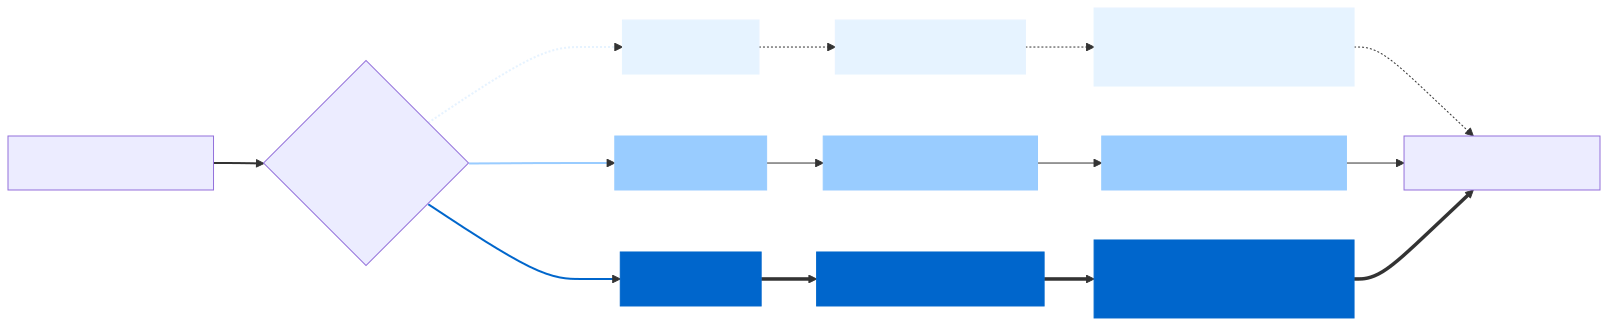
\includegraphics[width=10.41667in,height=5.20833in]{main_files/mediabag/illustrationen/lop_visualisierung.pdf}

Die durchgeführten Experimente bieten - wie so oft in der Psychologie -
nur Indizien. Aber es spricht vieles dafür, dass sich das auch auf das
Lernen übertragen lässt. Häufiges Repetieren kann zu einer Lernillusion
führen. Die Repetitionen bleiben ausschliesslich in der phonlogischen
Schlaufe (Werbung Glückspost - eine Mark), schaffen es aber nicht ins
Langzeitgedächtnis.

\subsection{Methodisches}\label{methodisches}

Wie habe ich versucht, meine Arbeitshypothese zu überprüfen?

\begin{itemize}
\tightlist
\item
  Natürliches Experiment
\item
  Leitfadeninterview
\item
  Auswertung erbrachter Leistungen
\end{itemize}

\subsection{Natürliches Experiment}\label{natuxfcrliches-experiment}

\begin{tcolorbox}[enhanced jigsaw, opacityback=0, arc=.35mm, coltitle=black, opacitybacktitle=0.6, title={Charakteristik}, bottomrule=.15mm, colbacktitle=quarto-callout-note-color!10!white, toprule=.15mm, bottomtitle=1mm, breakable, toptitle=1mm, left=2mm, rightrule=.15mm, leftrule=.75mm, colframe=quarto-callout-note-color-frame, titlerule=0mm, colback=white]

\begin{itemize}
\tightlist
\item
  Ersatz für ein Laborexperiment
\end{itemize}

\end{tcolorbox}

\begin{tcolorbox}[enhanced jigsaw, opacityback=0, arc=.35mm, coltitle=black, opacitybacktitle=0.6, title={Zu bedenken}, bottomrule=.15mm, colbacktitle=quarto-callout-warning-color!10!white, toprule=.15mm, bottomtitle=1mm, breakable, toptitle=1mm, left=2mm, rightrule=.15mm, leftrule=.75mm, colframe=quarto-callout-warning-color-frame, titlerule=0mm, colback=white]

\begin{itemize}
\tightlist
\item
  Muss entdeckt werden
\item
  Beinhaltet viele Störvariabeln
\end{itemize}

\end{tcolorbox}

Die Kontrollgruppe war besser als die Testgruppe.

\subsection{Leitfadeninterview}\label{leitfadeninterview}

\begin{tcolorbox}[enhanced jigsaw, opacityback=0, arc=.35mm, coltitle=black, opacitybacktitle=0.6, title={Charakteristika}, bottomrule=.15mm, colbacktitle=quarto-callout-note-color!10!white, toprule=.15mm, bottomtitle=1mm, breakable, toptitle=1mm, left=2mm, rightrule=.15mm, leftrule=.75mm, colframe=quarto-callout-note-color-frame, titlerule=0mm, colback=white]

\begin{itemize}
\tightlist
\item
  Qualitative Methode
\item
  Systematische Auswertung der gewonnenen Information
\end{itemize}

\end{tcolorbox}

\begin{tcolorbox}[enhanced jigsaw, opacityback=0, arc=.35mm, coltitle=black, opacitybacktitle=0.6, title={Zu bedenken}, bottomrule=.15mm, colbacktitle=quarto-callout-warning-color!10!white, toprule=.15mm, bottomtitle=1mm, breakable, toptitle=1mm, left=2mm, rightrule=.15mm, leftrule=.75mm, colframe=quarto-callout-warning-color-frame, titlerule=0mm, colback=white]

\begin{itemize}
\tightlist
\item
  Schwierig, geeignete Gesprächssituationen zu schaffen
\end{itemize}

\end{tcolorbox}

Weil ich als Lehrer das Interview geführt habe, ist kein
herrschaftsfreier Diskurs im Sinne Habermas' zustandegekommen.

\subsection{Auswertung erbrachter
Leistungen}\label{auswertung-erbrachter-leistungen}

\begin{tcolorbox}[enhanced jigsaw, opacityback=0, arc=.35mm, coltitle=black, opacitybacktitle=0.6, title={Charakteristika}, bottomrule=.15mm, colbacktitle=quarto-callout-note-color!10!white, toprule=.15mm, bottomtitle=1mm, breakable, toptitle=1mm, left=2mm, rightrule=.15mm, leftrule=.75mm, colframe=quarto-callout-note-color-frame, titlerule=0mm, colback=white]

\begin{itemize}
\tightlist
\item
  Grösserer Datenumfang
\item
  Unterschiedliche Auswertungen möglich
\end{itemize}

\end{tcolorbox}

\begin{tcolorbox}[enhanced jigsaw, opacityback=0, arc=.35mm, coltitle=black, opacitybacktitle=0.6, title={Zu bedenken}, bottomrule=.15mm, colbacktitle=quarto-callout-warning-color!10!white, toprule=.15mm, bottomtitle=1mm, breakable, toptitle=1mm, left=2mm, rightrule=.15mm, leftrule=.75mm, colframe=quarto-callout-warning-color-frame, titlerule=0mm, colback=white]

\begin{itemize}
\tightlist
\item
  Sekundärdaten passen nicht exakt zur Fragestellung
\end{itemize}

\end{tcolorbox}

Resultate kommen

\subsection{Resultate}\label{resultate}

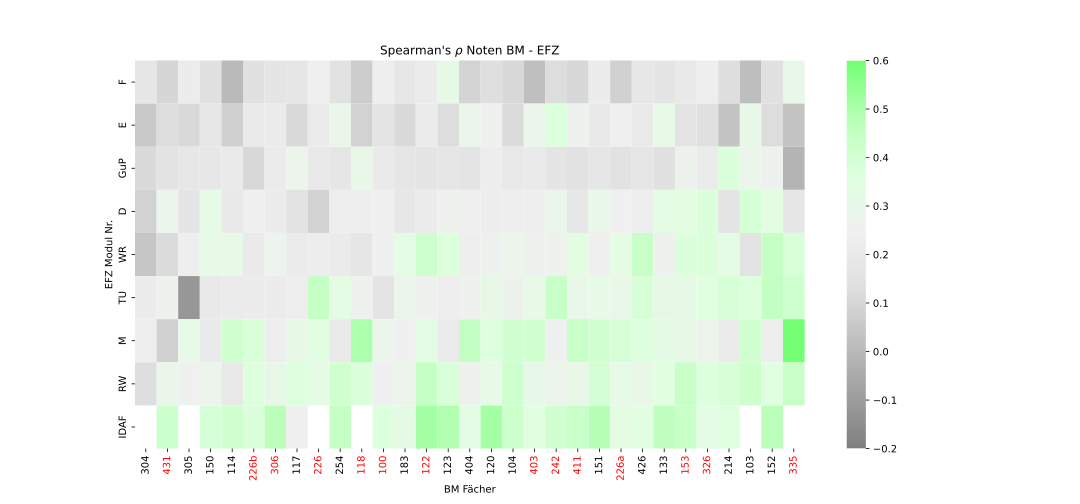
\includegraphics{main_files/mediabag/illustrationen/spearman_heatmap.pdf}

IDAF als unvollständiger Datensatz entfernt. Wenn die Arbeitshypothese
zutreffen würde, müssten die rot eingefärbten Modulnummern rechts
stehen.

\subsection{Resultate}\label{resultate-1}

\includegraphics{illustrationen/gw.png}
\includegraphics{illustrationen/sw.png}
\includegraphics{illustrationen/aw.png}

Unterstreicht, was bereits die Heatmap gezeigt hat.

\subsection{}\label{section}

\begin{tcolorbox}[enhanced jigsaw, opacityback=0, arc=.35mm, coltitle=black, opacitybacktitle=0.6, title={Feststellung}, bottomrule=.15mm, colbacktitle=quarto-callout-important-color!10!white, toprule=.15mm, bottomtitle=1mm, breakable, toptitle=1mm, left=2mm, rightrule=.15mm, leftrule=.75mm, colframe=quarto-callout-important-color-frame, titlerule=0mm, colback=white]

Die Arbeitshypothese konnte weder bestätigt noch widerlegt werden.

\end{tcolorbox}

\subsection{Folgerungen}\label{folgerungen}

\begin{tcolorbox}[enhanced jigsaw, opacityback=0, arc=.35mm, coltitle=black, opacitybacktitle=0.6, title={Konsequenzen für den Unterricht}, bottomrule=.15mm, colbacktitle=quarto-callout-note-color!10!white, toprule=.15mm, bottomtitle=1mm, breakable, toptitle=1mm, left=2mm, rightrule=.15mm, leftrule=.75mm, colframe=quarto-callout-note-color-frame, titlerule=0mm, colback=white]

\begin{itemize}
\tightlist
\item
  Es gibt keine überlegene Unterrichtsmethode
\item
  Entscheidend ist die Methodenvielfalt
\end{itemize}

\end{tcolorbox}

\subsection{Persönliche Erkenntnisse}\label{persuxf6nliche-erkenntnisse}

\begin{itemize}
\tightlist
\item
  Quantitative sozialwissenschaftliche Studien sind mit Vorsicht zu
  geniessen
\item
  Qualitativen Argumente haben eine eigene Überzeugungskraft
\item
  Die Wahl geeigneter Visualisierungen ist entscheidend
\item
  Die Schweiz ist ein didaktisches Entwicklungsland
\end{itemize}

Die persönlichen Erkenntnisse reichen über das Thema der Arbeit hinaus.

\begin{enumerate}
\def\labelenumi{\arabic{enumi}.}
\tightlist
\item
  Oft sind die Stichproben sehr klein. Es gibt sehr viele Störvariabeln.
\item
  Als Geisteswissenschaftler muss man sich auch auf die Kraft der
  Argumente verlassen.
\item
  Die angetroffenen inhaltlichen Studien stammen aus Ländern, denen man
  didaktische Forschung gar nicht zugetraut hätte.
\end{enumerate}

\subsection{}\label{section-1}

\begin{tcolorbox}[enhanced jigsaw, opacityback=0, arc=.35mm, coltitle=black, opacitybacktitle=0.6, title={Fazit}, bottomrule=.15mm, colbacktitle=quarto-callout-warning-color!10!white, toprule=.15mm, bottomtitle=1mm, breakable, toptitle=1mm, left=2mm, rightrule=.15mm, leftrule=.75mm, colframe=quarto-callout-warning-color-frame, titlerule=0mm, colback=white]

Ich würde es wieder machen.

\end{tcolorbox}




\end{document}
